\documentclass[12pt]{article}
\usepackage{amsmath,amssymb}
\usepackage[utf8]{inputenc}
\usepackage{textcomp}
\usepackage{times}
\usepackage[margin=1in]{geometry}
\usepackage{setspace}
\usepackage{longtable}
\usepackage{booktabs}
\usepackage{titlesec}
\usepackage{needspace}
\usepackage{etoolbox}
\usepackage{enumitem}  % For custom bibliography numbering
\usepackage{graphicx}
\usepackage{url}
\providecommand{\tightlist}{}   % makes \tightlist a harmless no-op
\providecommand{\pandocbounded}[1]{#1}   % simply passes its argument through

\usepackage[x11names]{xcolor}
\definecolor{DarkGreen}{rgb}{0,0.4,0}

% … later, replace your hyperref line with:
\usepackage[colorlinks=true,
            citecolor=DarkGreen,
            linkcolor=DarkGreen,
            urlcolor=DarkGreen]{hyperref}


% ——— URL/DOI wrapping ———
\usepackage{xurl}                 % smarter line breaks in long URLs
\urlstyle{same}

% ——— CSL-generated bibliography ———
% ——— CSL-generated bibliography ———
\newlength{\cslhangindent}
\setlength{\cslhangindent}{3.5em}

\newenvironment{CSLReferences}[2]%
  {\begin{enumerate}[label={[\arabic*]}, leftmargin=100pt, labelwidth=*, labelsep=0.5em, itemsep=5pt]%
   \raggedright\sloppy}%
  {\end{enumerate}}

\providecommand{\CSLLeftMargin}[1]{\item}   % starts the list item
\providecommand{\CSLRightInline}[1]{#1}     % prints the entry text


% —— Hyperref must be loaded LAST with correct options ——
\usepackage[colorlinks=true]{hyperref}
\urlstyle{same}

% —— Section formatting ——
\setcounter{secnumdepth}{3}
\titleformat{\section}[hang]
  {\normalfont\Large\bfseries}
  {\thesection.}{1em}{}
\titleformat{\subsection}[hang]
  {\normalfont\large\bfseries}
  {\thesubsection.}{1em}{}
\titlespacing*{\section}{0pt}{*2}{*0.5}
\titlespacing*{\subsection}{0pt}{*1.5}{*0.6}

% —— Critical citeproc fixes ——
\makeatletter
\protected\def\citeproctext{}
\let\@oldprotect\protect
\def\@citeprocprotection{\let\protect\@oldprotect}
\protected\def\citeproc{}
\protected\def\citeprocfootnote#1{\footnote{#1}}
\makeatother

% —— Figure settings ——
\setkeys{Gin}{keepaspectratio,height=0.85\textheight,width=\linewidth}
\makeatletter\def\fps@figure{htbp}\makeatother
\graphicspath{{figures/}}
\newcommand{\sectionbreak}{\vspace{1\baselineskip}}

% —— Special character definitions ——
\DeclareUnicodeCharacter{2203}{\ensuremath{\exists}}
\DeclareUnicodeCharacter{2200}{\ensuremath{\forall}}
\DeclareUnicodeCharacter{2227}{\ensuremath{\wedge}}
\DeclareUnicodeCharacter{2228}{\ensuremath{\vee}}
\DeclareUnicodeCharacter{2192}{\ensuremath{\rightarrow}}
\DeclareUnicodeCharacter{2194}{\ensuremath{\leftrightarrow}}
\DeclareUnicodeCharacter{2234}{\ensuremath{\therefore}}
\DeclareUnicodeCharacter{2248}{\ensuremath{\approx}}

% —— Custom table support ——
\usepackage{array}
\usepackage{longtable}
\usepackage{calc}
\newcolumntype{C}[1]{>{\raggedright\arraybackslash}p{\dimexpr#1\linewidth-4\tabcolsep\relax}}

% —— Document metadata ——
\title{Patterns, Pragmatism, and Mild Realism. \\[0.5em] \large An Empirical Probe}
\author{Florin Cojocariu}
\date{06.05.2025}

\begin{document}

\maketitle

\begin{abstract}
This essay revisits the question of whether patterns in language are real, by comparing Daniel Dennett's ``mild-realism'' claim that patterns are real when they help us compress and predict information, with Norton Nelkin's instrumentalist view that patterns are interpretive constructs, not features of the world itself. I examine how words like \emph{cat}, \emph{hammer}, or \emph{water} create different \emph{patterns of use\footnote{All along this essay we'll see how the projections of sentences in a given sub-space create graphical patterns. But these visual patterns encode in reality \textbf{patterns of use}, something impossible for us to quantify without an LLM.}} when employed in different kinds of sentences.

By analyzing series of naturally occurring sentences with a given word by using sentence-embedding models,\footnote{SBERT obtains state-of-the-art performance on capturing sentence similarity and distributional semantics \cite{ref-milliereBuckner2024}.} I show that meaning forms around a word not as a fixed point but as a shape---with a dense, literal ``core'' of usage and a more variable, figurative ``halo.'' This structure emerges from the language itself, not from theoretical imposition, similarly to how a mountain is a real gradient in height, not an artifact of our measurement method.

My approach uses SBERT to classify naturally occurring sentences into literal (P-type) and idiomatic (Q-type) uses, mapping them into semantic space using role-based projections\footnote{Each axis (Agent ↔ Object, Literal ↔ Metaphoric, Perceived ↔ Symbolic, Quantity ↔ Quality, Thing ↔ Concept) was constructed from curated sentence pairs and achieves AUC \textgreater{} 0.9 on held-out tests \cite{ref-milliereBuckner2024}.}. The resulting sentence embeddings consistently reveal a distinctive shape: a dense, stable P-core surrounded by a looser Q-cap. I argue that P-cores satisfy Dennett's criteria for real patterns---they are stable, reproducible, and predictive---while Q-caps exhibit the variability that motivates Nelkin's skepticism but are nevertheless also ``real patterns''; in the end, the thesis here is that empirical evidence validates Dennett's view while it partly contradicts Nelkin's skepticism.

Philosophically, this discovery of a spectrum from literal, sensory uses to idiomatic uses suggests a solution to ancient puzzles about how words ``hook'' into reality, showing that concepts are not atomic objects but fluid patterns with stable cores and shifting halos.
\end{abstract}
\vspace{1em}

\setcounter{tocdepth}{3}
\section{Introduction}\label{introduction}

What makes a pattern real? This question sits at the core of Daniel Dennett's influential 1991 paper \emph{Real Patterns}, which argues that a pattern is real if it enables compression and predictive power---if it ``pays for the cost of its own description'' \cite{ref-dennettRealPatterns1991}. Norton Nelkin (1994) counters that patterns, especially in scientific or linguistic domains, are epistemic conveniences, not ontological commitments: they reflect how we organize the world, not how the world is \cite{ref-nelkinPatterns1994}. I use their debate as a starting point for studying patterns in LLM sentence embeddings. The reasoning is founded on the idea that words are acquired first as simple labels for patterns of sensations.\footnote{Infant studies show that word learning is driven by perceptual salience and multisensory input and because of that, words function as pure 'labels' when first employed. \cite{ref-hollichBreaking2000,ref-prudenBirth2006,ref-seidlTouch2024}.} ``Cat'' is, at first, just a label for a shape, a texture, some specific sounds. I call this primitive label-usage the ``object-word.''

My method may seem an unusual one, as it blends philosophical work with concrete empirical observations on the internal structure of a Large Language Model (SBERT). It is my view that LLMs are exceptional research objects of a new kind, offering us a new testing ground for the philosophy of language. In this case, we can literally see how (and why) Wittgenstein's ``meaning is use'' is true.

I target first multiple sentences containing specific object-words like \emph{cat}, \emph{fork}, \emph{tomato}, the assumption being that their distribution in the embedding space will reflect through certain patterns the way we use the words. For each word, I build then a corpus of naturally occurring sentences and classify them into P-type (literal, concrete use) and Q-type (figurative, idiomatic use). Projected into 2D space, the embeddings reveal a consistent topological form: a dense stem-like cluster of literal sentences (the rod), surrounded by a diffuse cap of idiomatic uses (the mushroom). A couple of additional dimensions can be identified and make a projection in 3D where the patterns that certain uses of the word emerge more clearly.

An extensive description of the method and links to relevant scripts used to analyze the data in SBERT can be found in the long form essay.

\section{From Words to Space: Semantic Embeddings and Role Axes}\label{from-words-to-space-semantic-embeddings-and-role-axes}

The empirical approach hypothesized at first five cardinal directions that track familiar philosophical contrasts---``semantic axes'': Agent ↔ Object, Literal ↔ Metaphoric, Perceived ↔ Symbolic, Quantity ↔ Quality, Thing ↔ Concept. Every sentence can be located by a five-number ``role vector,'' revealing its blend of agency, literality, and so on \cite{ref-milliereBuckner2024}. We classified manually some test sentences with ``cat'' and we looked at their projection patterns along these axes.

As our axes are arbitrary at first, they simply serve as an initial reference system for projection but it is important to note that once the reference set is established, composite real axes that maximize the gradient of the distribution can be identified.

One such composite axis---angled toward both Thing vs.~Sign and Literal vs.~Metaphoric---seems to capture the main corridor along which meaning slides from concrete usage into idiom and displayed a clear emerging pattern. I call this the ``real axis'' because it captures a familiar philosophical journey: from showing to saying, from concrete to concept.

To test the idea, I constructed two contrasting sentence sets:
- **Proust Set**: sensory, phenomenal uses (e.g.~``the candle flickered'')
- **Quine Set**: abstract, symbolic uses (e.g.~``the candle represents hope'')

The separation proved clear and measurable.\footnote{Principal-component analysis and centroid-distance metrics show high separation between Proust vs.~Quine sentences in the 5D role space (AUC \textgreater{} 0.9) \cite{ref-milliereBuckner2024}.}

\section{Our Model: Rods and Caps}\label{our-model-rods-and-caps}

While certain precautions were employed to make sure we're not finding artifacts generated by the method, more extensive testing (using different models) is needed to fully validate the results. However, we've seen how, across many examples, literal sentences huddle tightly around a center, like a slender rod\footnote{At this stage it is more like a point, but later on, when we switch to 3D and we discover how definition sentences project, this emerges as an elongated feature.} and figurative sentences spread outward in wide, overlapping caps. The pattern seemed robust: rods stay compact, caps diffuse, and led us to proposing a model for this type of pattern:

**Rods (P-sentences)**: Embeddings of literal usages cluster tightly near the word's core meaning, forming a small, centered ``rod'' with high pairwise cosine similarities (mean ≈ 0.83) and low variance \cite{ref-parkGeometry2025}---highly compressible and repeatable across contexts.

**Caps (Q-sentences)**: Embeddings of figurative usages scatter outward in many directions, forming broad ``caps'' that occupy multi-lobed shapes, overlap arbitrarily with other words' caps, and resist systematic compression (mean pairwise cosine similarity ≈ 0.46) \cite{ref-parkGeometry2025}.

There is extensive literature on children acquiring language that seems to confirm the idea that P-sentences form `the core' of how a word is used at first in its `label' (or `object-word') function, while Q-sentences are uses acquired later on, when idiomatic and metaphorical uses start to be employed\footnote{\cite{ref-hollichBreaking2000,ref-prudenBirth2006,ref-seidlTouch2024}.}. There is an intriguing connection here to cognitive studies but this exceeds our scope which remains philosophical at its core: are our sentence patterns in the semantic space `real patterns'?

\subsection{Object-word and word-concept}\label{object-word-and-word-concept}

In our model we can introduce two constructions, defined first as the centroids of the two different distributions:
- **object-word**, as the centroid of the P sentences distribution, giving the `core' of the distribution of all literal use sentences. This usage is primary and can be seen as a `label' use without attached conceptual meaning; it simply describes properties of the corresponding object, like in ``cat meows''.
- **word-concept**, as a name for the entire cap formed by idiomatic, metaphoric and non-literal use sentences, like ``he let the cat out of the bag''. On a meta-level, both object-word and word-concept are labels for two different patterns we can see in an LLM sentence embedding space.

\subsection{Some empirical findings}\label{some-empirical-findings}

Below I have attached 3 graphs that resulted from the projection of different sentences in a subspace that includes the ``real axis.'' In the first one, a cylindrical projection is employed to analyze the distribution of P/Q sentences for different words. The P rods emerge (more clearly for some words than for others) and also the more fuzzy, distanced Q cap can be seen\footnote{In this specific image there are some artifacts, but further work eliminated most of them (possible model biases as in \cite{ref-lavieInfiniteSymmetry2024,ref-vasileiouBiLRP2024,ref-wenPrototype2025}). This is work in progress, and more in-depth testing and research is needed to fully confirm these results. But for the purposes of this essay, they seem real enough.}.

\begin{figure}
\centering
\pandocbounded{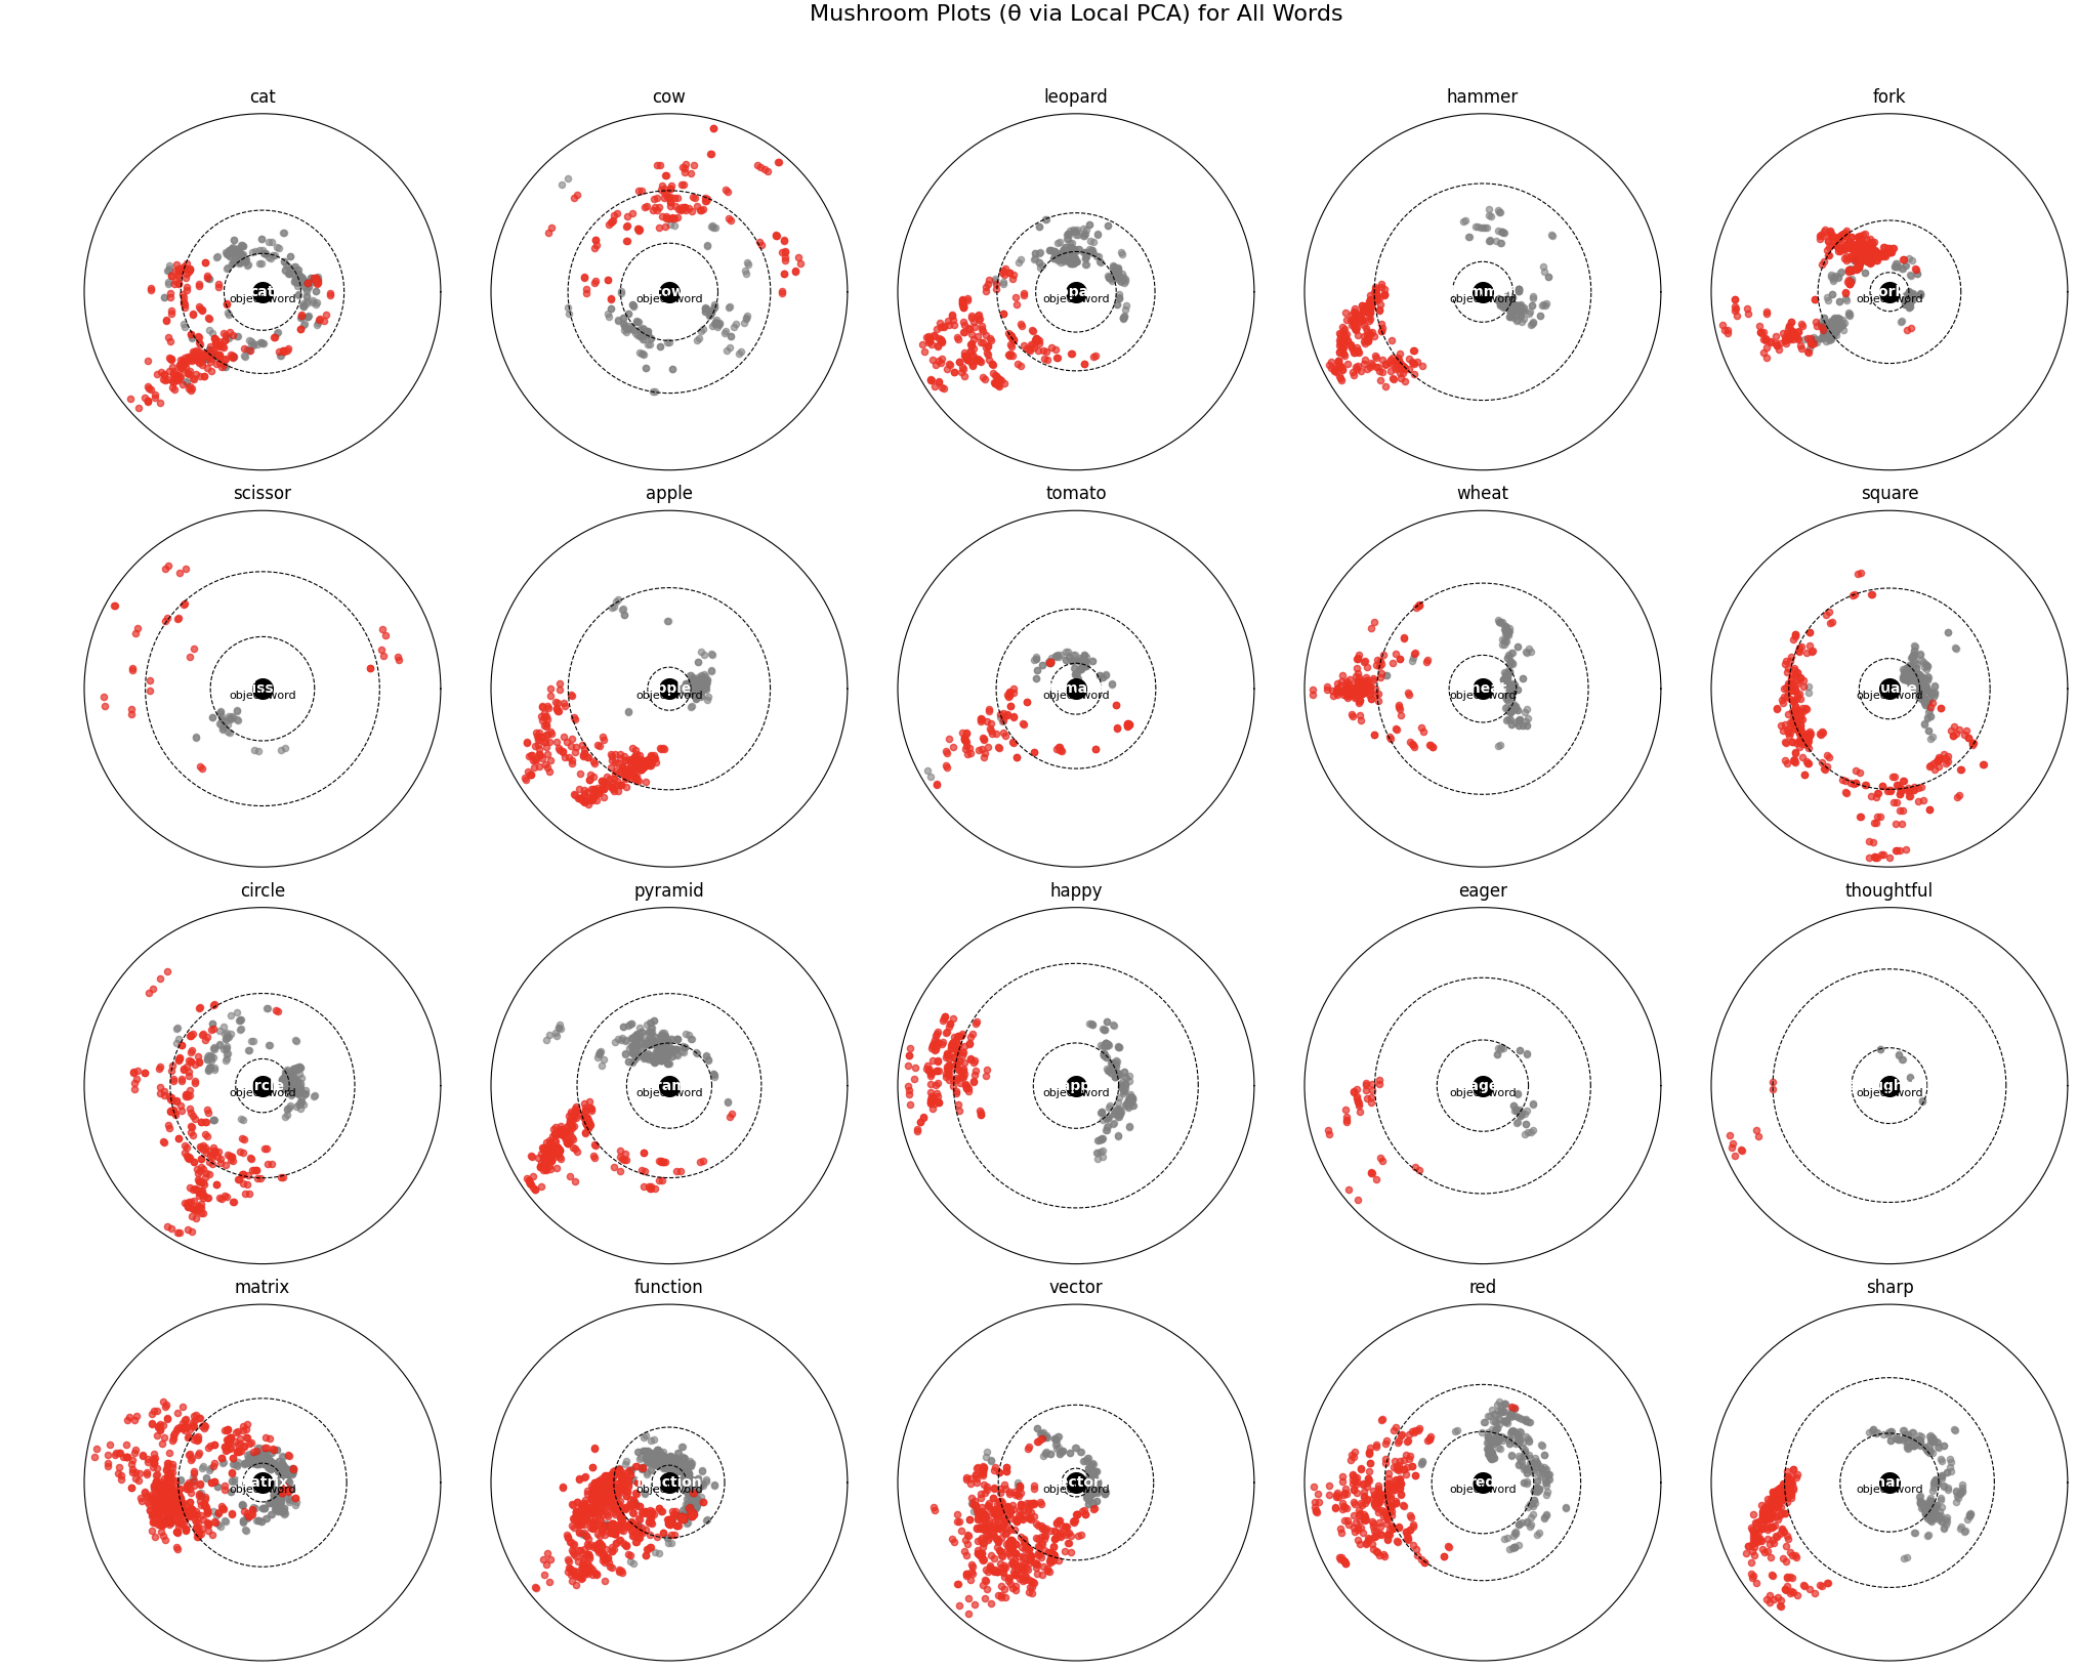
\includegraphics[keepaspectratio]{figures/rods_and_caps.png}}
\caption{Caps and Rods}
\end{figure}

The second one shows how ``cat'' and ``tomato'', despite overlapping their Q caps, have only one common sentence in our specific set, while ``cat'' and ``fork'' overlap but have none in common. This indicates the potential for non-literal, metaphoric use of the words in Q-cap sentences. For instance, ``A cat is a furred fork'' seems not so completely absurd because there is actual already potential overlap:

\begin{figure}
\centering
\pandocbounded{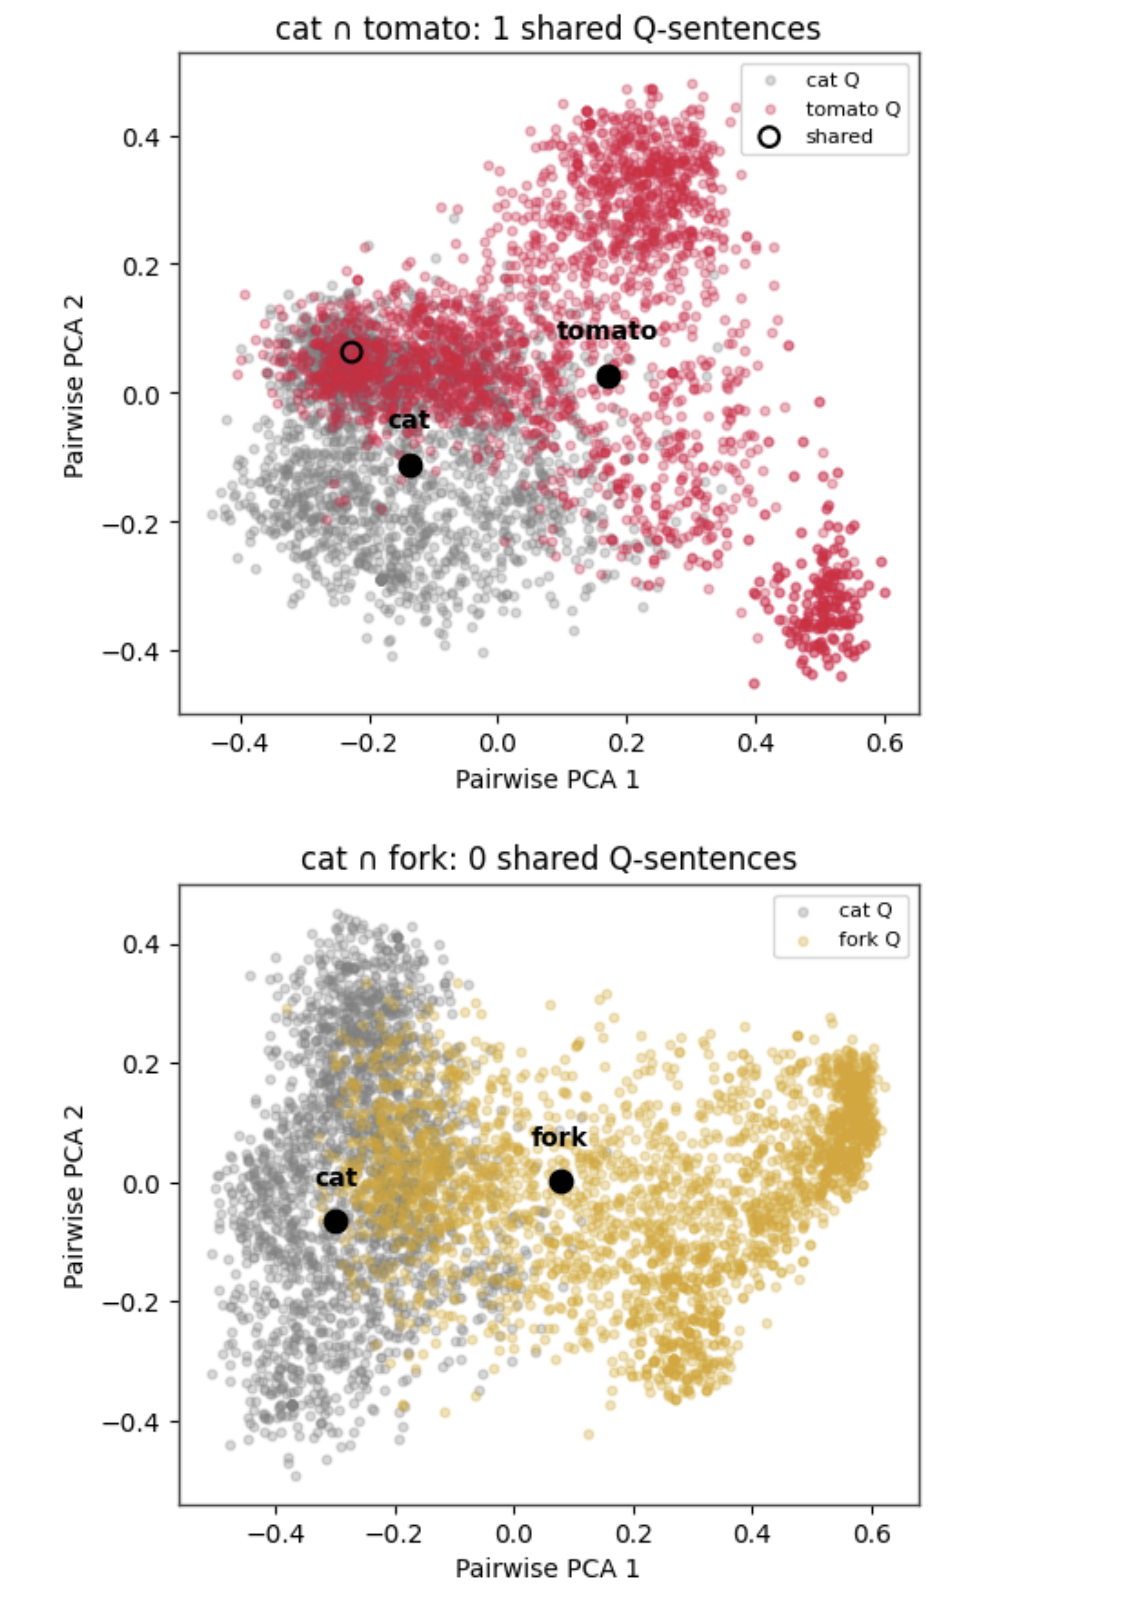
\includegraphics[keepaspectratio]{figures/caps.png}}
\caption{Overlapping Caps}
\end{figure}

The last graph plots the distinct area where definition sentences (their different types) can be found. In a 3D graph this is more striking, as they are far above most of the P and Q type sentences, suggesting a third ``abstraction'' axis in the semantic space, one is the actual ``rod'' that we talk about here, connecting literal, ``label'' word use to its most absolute abstraction (more about this below).

\begin{figure}
\centering
\pandocbounded{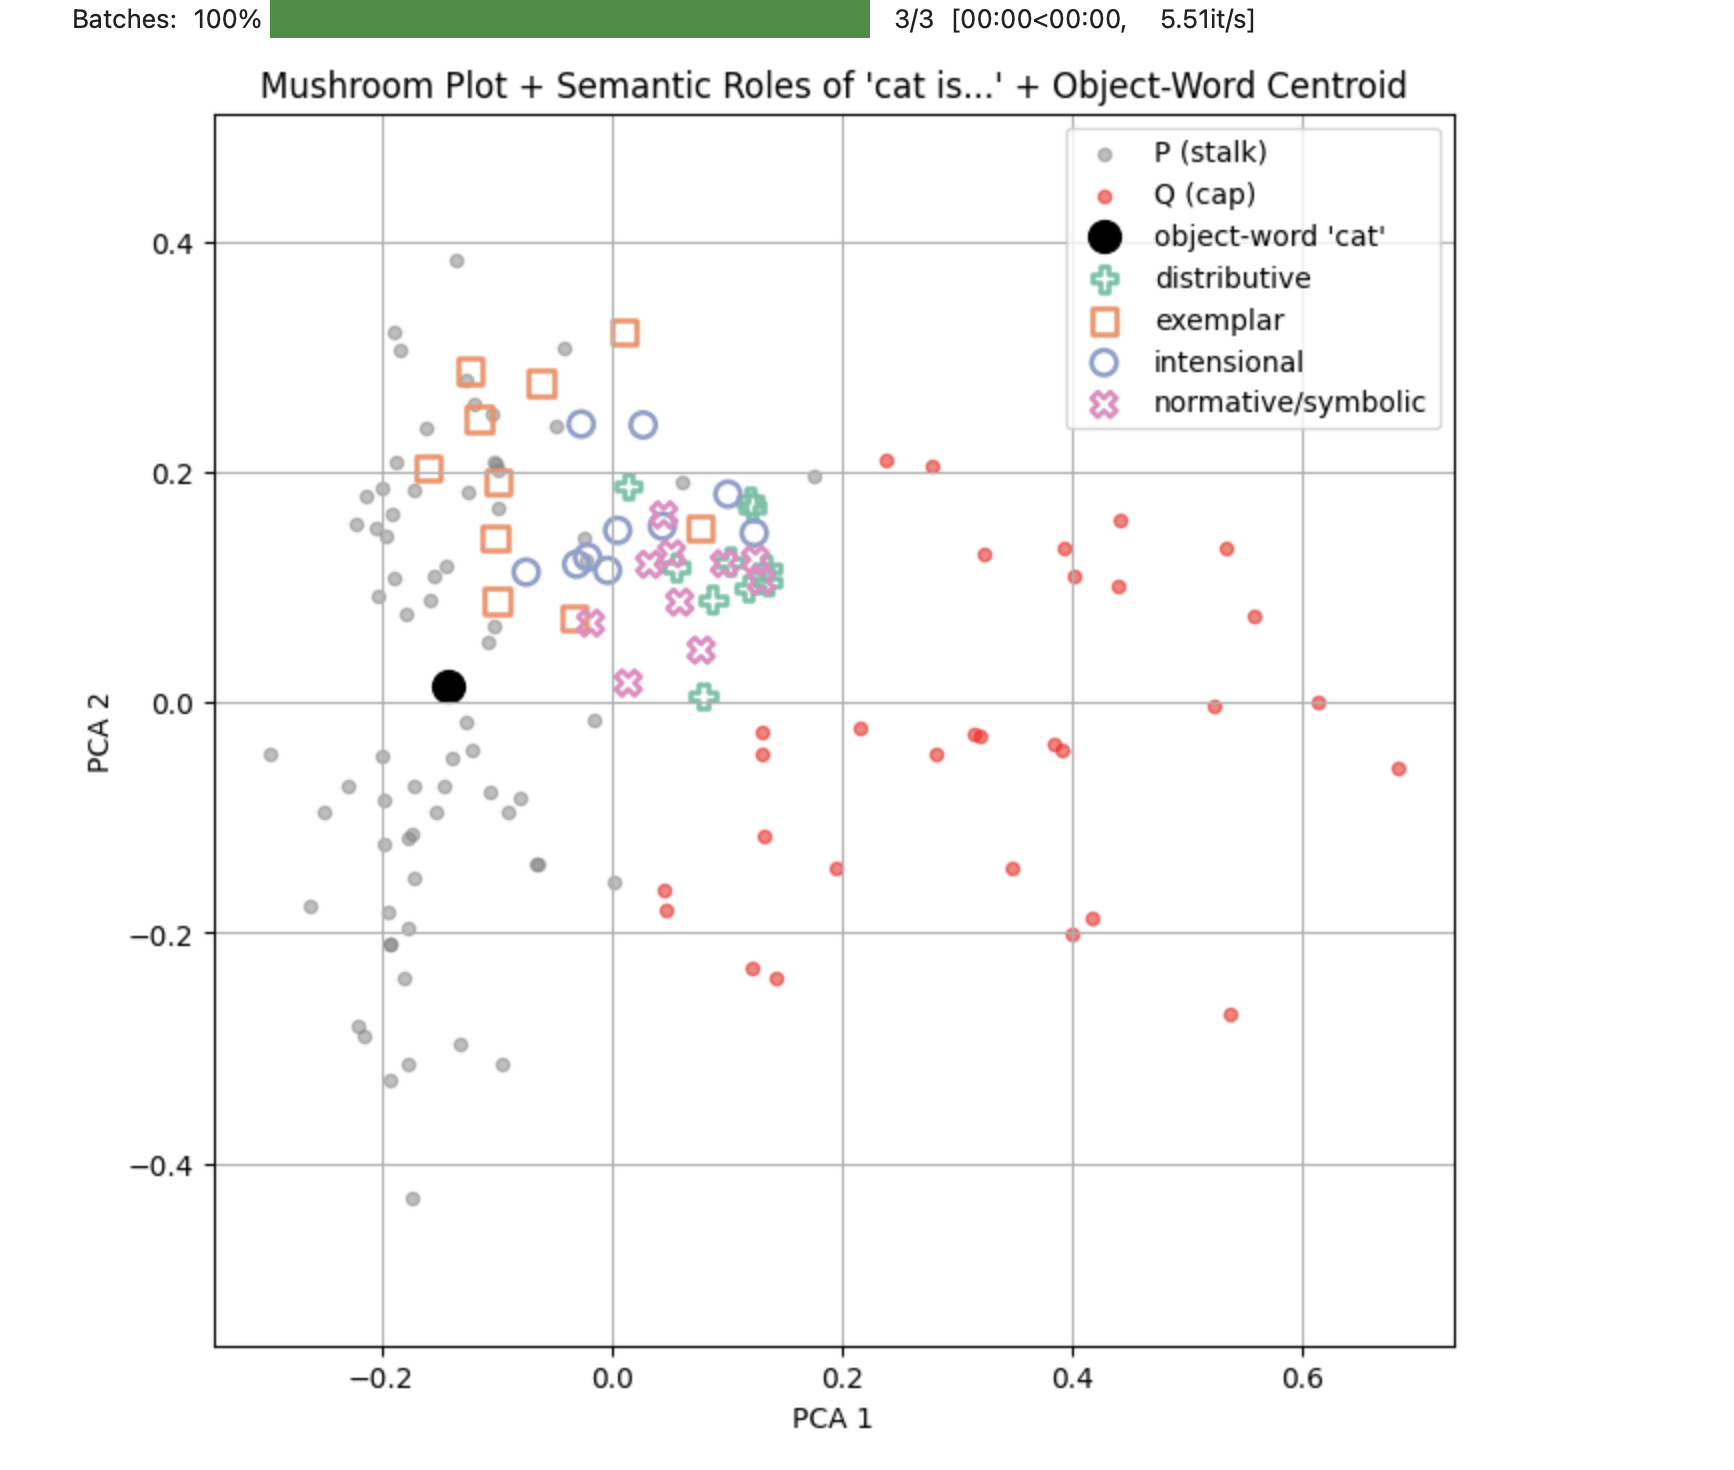
\includegraphics[keepaspectratio]{figures/definitions.png}}
\caption{Definitions}
\end{figure}

\subsection{Rods and Dennett's Real Patterns}\label{rods-and-dennetts-real-patterns}

Dennett (1991) defines real patterns by their compressibility, predictive power, and generality \cite{ref-dennettRealPatterns1991}. The rod-clusters satisfy each of these criteria. First, they are highly compressible: once the pattern is defined by a number of sentences, they contain in a small semantic space a very large quantity of information. If one asks you ``what a cat is?'' you can point them to this limited area in the semantic space where they'll find all possible literal sentences with ``cat''. In this sense, the object-word `cat' offers the maximum compression possible to send a staggering amount of information which all literal-use sentences with `cat' constitute \cite{ref-parkGeometry2025}. Second, rods have predictive utility---knowing a rod-pattern helps predict the expected behavior of the real objects they designate. Finally, rods generalize: the same compact structure reappears across different corpora and models \cite{ref-parkGeometry2025}.

Dennett certainly does not hold that spoken or written words are fixed, atomic entries. Instead, he writes:

\begin{quote}
``The process that produces the data of folk psychology, we claim, is one in which the multidimensional complexities of the underlying processes are projected through linguistic behavior, which creates an appearance of definiteness and precision, thanks to the discreteness of words.'' \cite{ref-dennettRealPatterns1991}
\end{quote}

Our model may be a good representation for this ``multidimensional complexities projection''. And, immediately thereafter, quoting Churchland's formulation of the same point:

\begin{quote}
``A person's declarative utterance is a `one-dimensional projection---through the compound lens of Wernicke's and Broca's areas---onto the idiosyncratic surface of the speaker's language---a one-dimensional projection of a four- or five-dimensional `solid' that is an element in his true kinematic state.'' \cite{ref-churchlandNeurocomputational2000}
\end{quote}

These passages show that for Dennett a word functions not as a static token but as a focal ``projection'' or ``center of gravity'' within a far richer, higher-dimensional pattern of cognitive and behavioral regularities; in other words, as a \emph{real} pattern.

\subsection{Caps and Nelkin's Anti-Realism}\label{caps-and-nelkins-anti-realism}

Nelkin (1994) argues that we cannot recognize a belief-pattern until we already possess the relevant propositional-attitude concepts---making the concept epistemically prior to the pattern \cite{ref-nelkinPatterns1994}:

\begin{quote}
``Of course, in some sense, until we have a concept of anything, X, we cannot sort instances under X. But, here, I am claiming something stronger. For instance, presumably, experiencing cats is relevant to our acquiring the concept `cat'. Only because we perceive token cats, patterned as cats, are we able to acquire the concept 'cat'. But the claim here is that we cannot even discern token belief-patterns (as patterns) until after we already possess propositional-attitude concepts. If so, the existence of the patterns can hardly give rise to our propositional-attitude concepts. To claim that the concepts originate from observing the patterns would have it upside down.''
\end{quote}

But in my rod/cap framework, this chicken-and-egg structure is avoided entirely. The rod is assembled empirically, as a body of appearances---sentences in which a word is used across diverse contexts. The cap emerges from the conceptual use of the word in different Q sentences (and this may correspond better to what Nelkin calls ``the concept cat'' above). These distributions do not change when we look from a different angle, they just \emph{appear} different; however, they may vanish if we choose a different set of semantic axes.

It is not that we see the pattern because we have the concept; rather, we form the concept because we encounter and respond to the pattern. Caps are not imposed by prior concepts but are stabilizations of functional use---resolvable from the rod without assuming prior interpretive categories.

Recent work on embedding geometry supports this: Lee et al.~2024 show that figurative or abstract meaning occupies nonlinear subspaces, while Park et al.~2025 demonstrate that literal category information resides in low-dimensional manifolds. Together, these findings imply that caps---rich in semantic nuance---must be diffuse and context-dependent (as Nelkin predicts), yet they remain empirically detectable as coherent clusters \cite{ref-leeGeometric2024,ref-parkGeometry2025}.

\subsection{Do we carry a LLM in our brains?}\label{do-we-carry-a-llm-in-our-brains}

The short answer is: not really. Our language is built over a much longer training period (up to 20 years) by being continuously immersed in the practice of language while experiencing reality. There may be some ``tight'' pattern formed by our neural network in association to literal uses of `cat'. But what I call `object-word' in a LLM may be a different beast from this pattern, because of our anchoring in reality and senses.

What we can see in an LLM is not what happens in our brain, but literally \emph{patterns of use} in language, specifically the fact that we use any word in two very different manners. An LLM is not reconstructing our mind or cognition; it simply looks for patterns in language, through vast amounts of text, close to all that humanity produced up to today\footnote{There is also the valid question of the reality anchor in LLMs. The ``object-word'' is simply a reconstruction, based on patterns of language use, that an LLM does for something truly connected to senses and reality in our mind \cite{ref-prudenBirth2006}.}.

\section{A Crucial Discovery: Definitions vs.~Literal Centers}\label{a-crucial-discovery-definitions-vs.-literal-centers}

Computing the centroid of the P set---the most perceptually grounded uses---gives an empirical anchor point for the object-word: a statistical center of the word's appearance across literal contexts. Interestingly, this centroid lies beneath and offset from the cluster of definitional sentences like ``A cat is a mammal,'' suggesting that intensional definitions are not the semantic core of the word, but rather a compressed projection that stabilizes certain generalizations. This aligns with Dennett's view that apparent precision of linguistic definition masks a much higher-dimensional pattern of cognitive regularity \cite{ref-fodorPsychosemantics1987,ref-churchlandNeurocomputational2000}\footnote{Fodor (1987) argues that intensional definitions often fail to capture the full variability of usage; Churchland (2000) describes how declarative utterances project a high-dimensional cognitive state into a single sentence.}. The object-word is not a fixed token or entry, but a center of gravity within a distributed field of appearances---a real pattern empirically discoverable through topological regularities in language use.

\section{Philosophical Conclusions}\label{philosophical-conclusions}

One important consequence derives from finding a literal vs.~idiomatic axis structuring any semantic corpus. This axis indicates a link to the ancient philosophical problem of how a word ``hooks'' into the real world and to the equally old problem of what ``concepts'' really are. My model suggests that there is a link between pre-verbal patterns of sensations with patterns of word usage in sentences, proposing a new definition for concepts.

A dual structure, with a hard core and a flexible halo acquired through time and experience, can be theorized for all sorts of patterns, including visual patterns. This may be possible because all our knowledge implies a connection from the outside world to our mind and lives always under the tension of ``hard, objective truth'' and ``personal, subjective interpretation.''

The pattern of the cap (i.e., the meaning of the word) is a pattern of sentences---a pattern of word use, acquired through use rather than definition. This approach offers solutions to some problems about meaning in general: how can meanings evolve and still be coherent? How can we have slightly different meanings for words and still communicate? It also sheds light on Quine's indeterminacy of translation: ``gavagai'' is not to be translated by observing actions but by looking at the pattern of sentences the word is used in.

My model shows that Dennett's mild realism description of patterns is closer to what actual patterns inside an LLM really are. It is difficult to understand the rod and cap distributions as conceptual artifacts in Nelkin's sense because they do not depend, as patterns, on the theoretical method we use to look at them.

\section{Limitations and Next Steps}\label{limitations-and-next-steps}

Finally, a few caveats and future directions:
\begin{itemize}
  \item \textbf{Architectural biases.} SBERT's transformer architecture may introduce its own clustering tendencies \cite{ref-lavieInfiniteSymmetry2024,ref-vasileiouBiLRP2024,ref-wenPrototype2025}. We need to verify whether literal/figurative splits reflect genuine usage or model-specific artifacts.
  \item \textbf{Human vs.~model Q-caps.} It remains to be seen whether Q-caps produced by speakers of a language share the same shape, suggesting objective structure, even when the exact sentence content differs across individuals. An experiment asking people to generate 30 ``cat'' sentences each and then mapping them to verify cross-speaker consistency would help settle this.
  \item \textbf{Generalizability.} While the rod/cap distinction holds across several words and domains, additional work---possibly including other embedding models---will test robustness.
\end{itemize}

\begin{center}\rule{0.5\linewidth}{0.5pt}\end{center}

\subsection*{Bibliography}\label{bibliography}

\subsubsection*{Primary Sources}
\begin{CSLReferences}{1}{0}
\bibitem[Dennett(1991)]{ref-dennettRealPatterns1991}
Dennett, Daniel C. 1991. "Real Patterns." \emph{The Journal of Philosophy} 88 (1): 27. doi:10.2307/2027085.

\bibitem[Nelkin(1994)]{ref-nelkinPatterns1994}
Nelkin, Norton. 1994. "Patterns." \emph{Mind \& Language} 9 (1): 56–87. doi:10.1111/j.1468-0017.1994.tb00216.x.
\end{CSLReferences}

\subsubsection*{Secondary Sources}
\begin{CSLReferences}{1}{0}
\bibitem[Churchland(2000)]{ref-churchlandNeurocomputational2000}
Churchland, Paul M. 2000. \emph{A Neurocomputational Perspective: The Nature of Mind and the Structure of Science}. Cambridge, MA: MIT Press.

\bibitem[Fodor(1987)]{ref-fodorPsychosemantics1987}
Fodor, Jerry A. 1987. \emph{Psychosemantics: The Problem of Meaning in the Philosophy of Mind}. Cambridge, MA: MIT Press.

\bibitem[Hollich et~al.(2000)]{ref-hollichBreaking2000}
Hollich, Gerhard, Kathy Hirsh-Pasek, Roberta M. Golinkoff, and Elizabeth A. Hennon. 2000. "Breaking the Language Barrier: An Emergentist Coalition Model for the Origins of Word Learning." \emph{Monographs of the Society for Research in Child Development} 65 (3): i–123.

\bibitem[Pruden et~al.(2006)]{ref-prudenBirth2006}
Pruden, Shannon M., Kathy Hirsh-Pasek, Roberta Michnick Golinkoff, and Elizabeth A. Hennon. 2006. "The Birth of Words: Ten-Month-Olds Learn Words Through Perceptual Salience." \emph{Child Development} 77 (2): 266–280. doi:10.1111/j.1467-8624.2006.00862.x.

\bibitem[Seidl et~al.(2024)]{ref-seidlTouch2024}
Seidl, Amanda H., Michelle Indarjit, and Arielle Borovsky. 2024. "Touch to Learn: Multisensory Input Supports Word Learning and Processing." \emph{Developmental Science} 27 (1): e13419. doi:10.1111/desc.13419.

\bibitem[Vasileiou and Eberle(2024)]{ref-vasileiouBiLRP2024}
Vasileiou, Christos, and Andrew Eberle. 2024. "Interpreting SBERT Similarity via BiLRP." \emph{Proceedings of the 2024 Conference on Empirical Methods in Natural Language Processing}.

\bibitem[Wen and Rezapour(2025)]{ref-wenPrototype2025}
Wen, Haoxin, and Yazdan Rezapour. 2025. "Prototype Layers Improve Figurative Language Detection in SBERT." \emph{Proceedings of the 2025 North American Chapter of the Association for Computational Linguistics}.
\end{CSLReferences}

\subsubsection*{Preprints}
\begin{CSLReferences}{1}{0}
\bibitem[Lavie et~al.(2024)]{ref-lavieInfiniteSymmetry2024}
Lavie, Jonathan, Shai Livnat, and Joshua Achiam. 2024. "Infinite Permutation Symmetry in Attention." \emph{Proceedings of the 2024 International Conference on Machine Learning}. (Preprint available on arXiv.)

\bibitem[Lee et~al.(2024)]{ref-leeGeometric2024}
Lee, Jin Hwa, Thomas Jiralerspong, Lei Yu, Yoshua Bengio, and Emily Cheng. 2024. "Geometric Signatures of Compositionality Across a Language Model's Lifetime." \emph{arXiv}. (Preprint.)

\bibitem[Millière and Buckner(2024)]{ref-milliereBuckner2024}
Millière, Raphaël, and Cameron Buckner. 2024. "A Philosophical Introduction to Language Models—Part I: Continuity with Classic Debates." \emph{arXiv}. (Preprint.)

\bibitem[Park et~al.(2025)]{ref-parkGeometry2025}
Park, Kiho, Yo Joong Choe, Yibo Jiang, and Victor Veitch. 2025. "The Geometry of Categorical and Hierarchical Concepts in Large Language Models." \emph{arXiv}. (Preprint.)
\end{CSLReferences}

\newcommand{\mylastpagefooter}{
  \thispagestyle{empty}
  \vspace*{\fill}
  \noindent\rule{\textwidth}{0.4pt}\\
  \noindent{\tiny florin.cojocariu@s.unibuc.ro, \today}
}
\AtEndDocument{\mylastpagefooter}

\end{document}